
\documentclass[11pt,letterpaper]{article}
\usepackage[english]{babel}
%\usepackage[ansinew]{inputenc}
\usepackage[utf8]{inputenc}
% \usepackage[latin1]{inputenc}
\usepackage[letterpaper,includeheadfoot, top=0.5cm, bottom=3.0cm, right=2.0cm, left=2.0cm]{geometry}
\renewcommand{\familydefault}{\sfdefault}

\usepackage{graphicx}
\usepackage{color}
\usepackage{hyperref}
\usepackage{amssymb}
\usepackage{url}
%\usepackage{pdfpages}
\usepackage{fancyhdr}
\usepackage{hyperref}
\usepackage{subfig}
\usepackage{listings}

\usepackage{listings} %Codigo
\lstset{language=C, tabsize=4,framexleftmargin=5mm,breaklines=true}

\newcommand*{\addheight}[2][.5ex]{%
  \raisebox{0pt}[\dimexpr\height+(#1)\relax]{#2}%
}

\begin{document}
\lstset{language=SQL}
%\begin{sf}
% --------------- ---------PORTADA --------------------------------------------
\newpage
%-------------------- CABECERA ---------------------
 
\includegraphics[scale=0.9]{img/logo.png}
%------------------ TÍTULO -----------------------
\vspace*{7cm}
\begin{center}
%\huge {Título Medio}\\
%\vspace{1cm}
\Large{CS5785 Applied Machine Learning - Fall 2017} \\
\vspace{3mm}
\huge{Homework 1}
\end{center}

%------------------ INFO -----------------------
\vfill
\begin{flushright}
\begin{minipage}{.45\linewidth}
\textbf{Team:} \hspace{5.5em} Navdeep Singh\\
\textcolor{white}{.} \hspace{8.1em} Vicente Rotman\\
\textbf{Professor:} \hspace{3.9em} Sergie Belongie\\
\textbf{Date:} \hspace{6.2em}09-13-2015 
\end{minipage}
\end{flushright}
\newpage


% ------------RESUMEN----------------------
\section{DigitRecognizer}
After downloaded the data from Digit Recognizer competition on Kaggle. Start working on the python code in the file named \textbf{digit\_recognizer.py}. The function called \textbf{main} open the file, it could be the test or train data and store all the data in 2 python lists. One called \textbf{labels\_test\_data} that has the labels of each digit and another called \textbf{test\_data} that stores the digits in the same order as the labels.
\subsection{b) Write a function to display an MNIST digit. Display one of each digit}
For this part there are 2 functions involved. The first one called \textbf{getOneSampleOfEachDigit(labels, data)} which returns a list with 10 digits, one of each option from 0 - 9. Then the other one is called \textbf{displayDigit(image)} this one receive the digit and plots it. Below there is the sample plot of each digit.
\\\\
\begin{tabular}{|c|c|c|c|}
      \hline
      \addheight{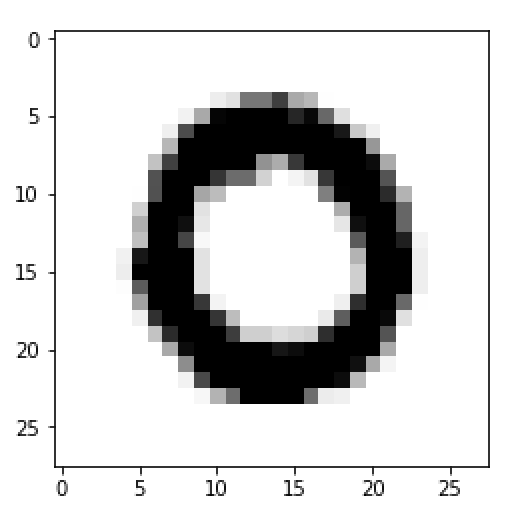
\includegraphics[width=30mm]{img/1-b/0.png}} &
      \addheight{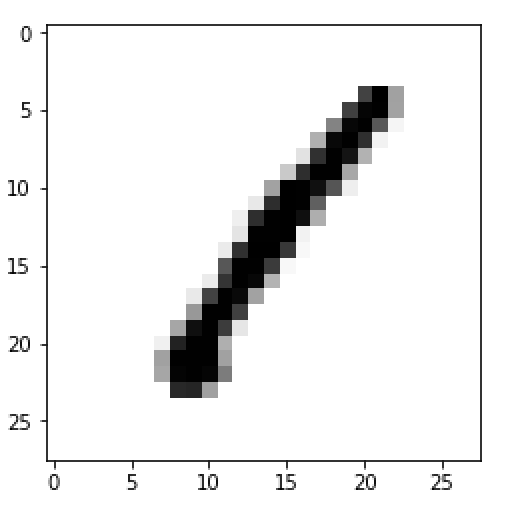
\includegraphics[width=30mm]{img/1-b/1.png}} &
      \addheight{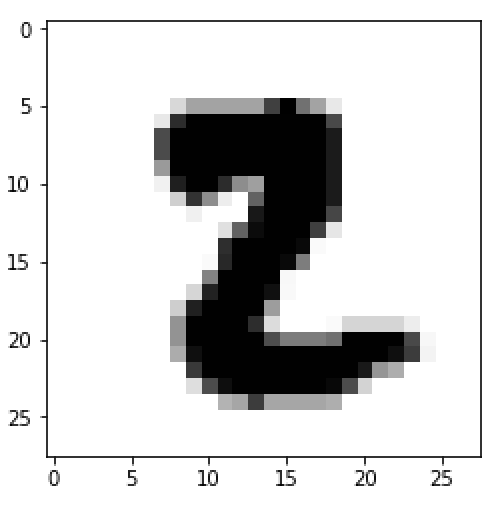
\includegraphics[width=30mm]{img/1-b/2.png}} &
      \addheight{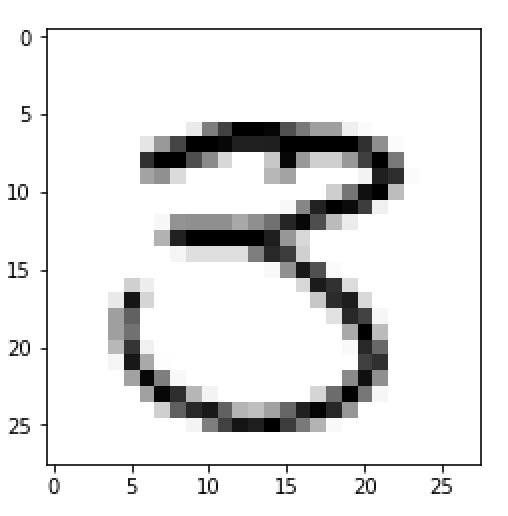
\includegraphics[width=30mm]{img/1-b/3.png}} \\
      \addheight{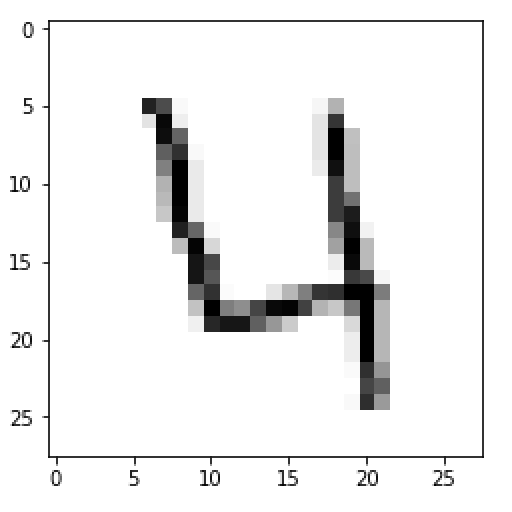
\includegraphics[width=30mm]{img/1-b/4.png}} &
      \addheight{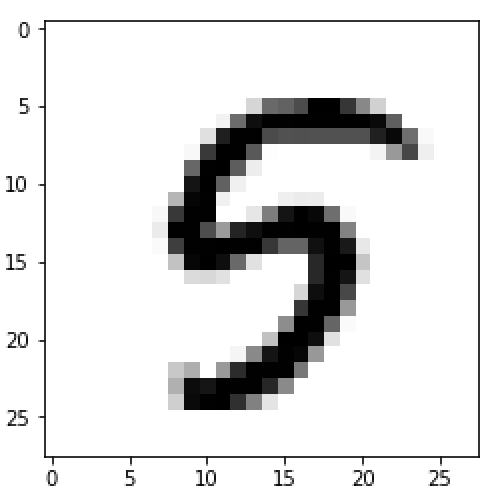
\includegraphics[width=30mm]{img/1-b/5.png}} &
      \addheight{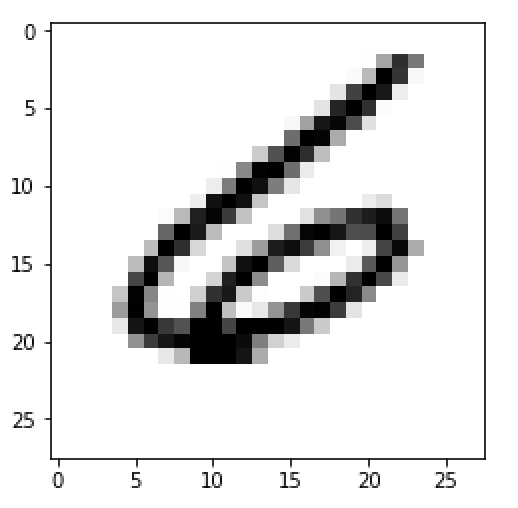
\includegraphics[width=30mm]{img/1-b/6.png}} &
      \addheight{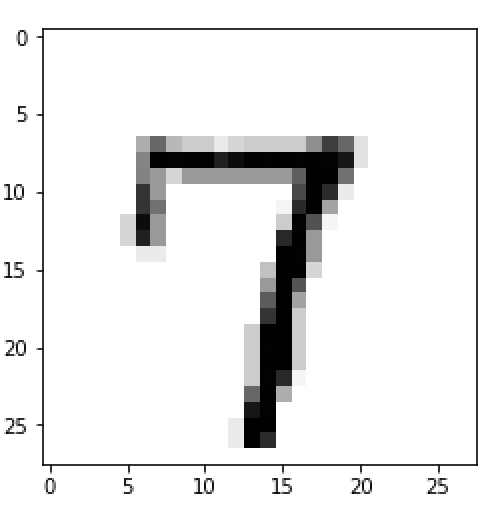
\includegraphics[width=30mm]{img/1-b/7.png}} \\
      \addheight{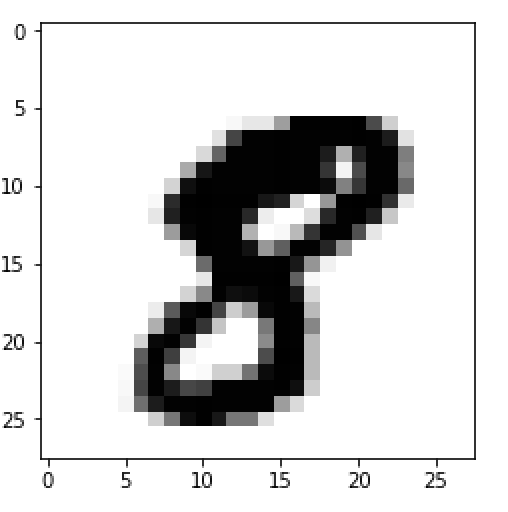
\includegraphics[width=30mm]{img/1-b/8.png}} &
      \addheight{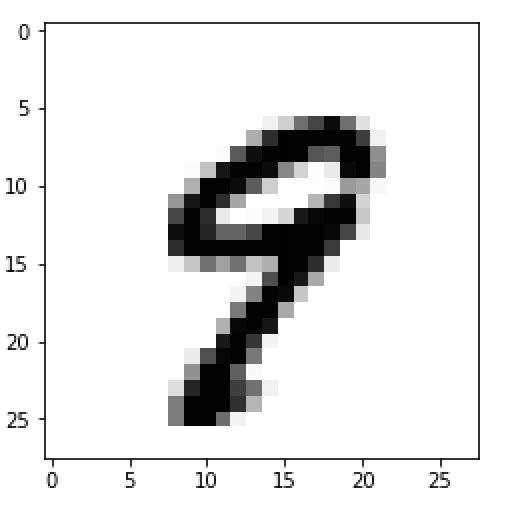
\includegraphics[width=30mm]{img/1-b/9.png}} \\
      \hline
\end{tabular}

\newpage
\subsection{c) Examine the prior probability of the classes in the training data. Is it uniform across the digits? Display a normalized histogram of digit counts. Is it even?}
To make the histogram, the only thing to do is to run a function called \textbf{displayHistogram(labels)}
Looking at the histogram below we can see that the distribution between the digits in enough uniform. We can say that is even.

\begin{figure}[ht!]
\centering
\fbox{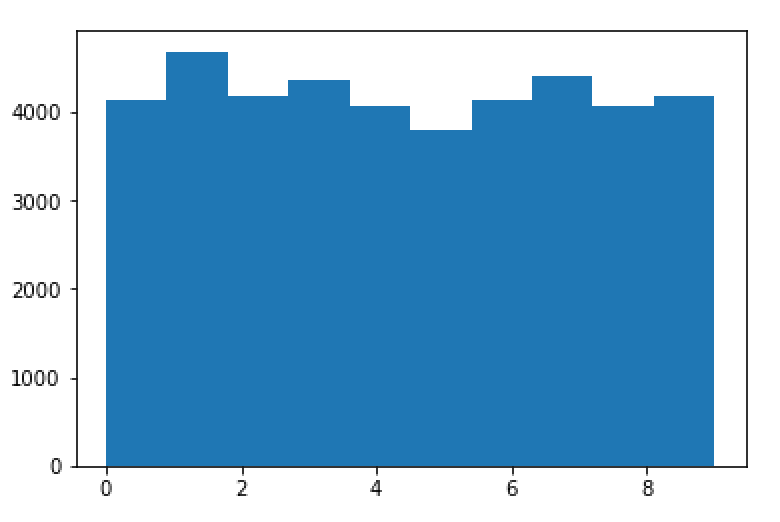
\includegraphics[scale=0.6]{img/1-c.png}}
\caption{Histogram of digit count}\label{Digit Count}
\end{figure}

\subsection{d) Pick one example of each digit from your training data. Then, for each sample digit, compute and show the best match (nearest neighbor) between your chosen sample and the rest of the training data. Use L2 distance between the two images’ pixel values as the metric. This probably won’t be perfect, so add an asterisk next to the erroneous examples (if any).}
To get sample of each digit there is a function in the python script called \textbf{getOneSampleOfEachDigit(labels, data)}, this returns an array with one sample of each digit. then for each one just run the function called \textbf{getNearestNeighbour(digit, data)}, this function compute the $L_2$ distance with the function \textbf{getDistance(first\_digit, second\_digit)} between the digit and all the other elements of the train data, then it returns the item with the smallest distance. This is the nearest neighbor, after that the function \textbf{displayDigit(image)}, plot the results. To run all of this there is the function \textbf{printNearestNeighbourOfEachDigit(labels, data)} that compute all the problem together and show the results in order, first the digit and then the neighbour. The results fit in all the cases except the number '3' which fails and show a number '5'. Below there is the results.

\begin{tabular}{|c|c|c|c|}
      \hline
      \addheight{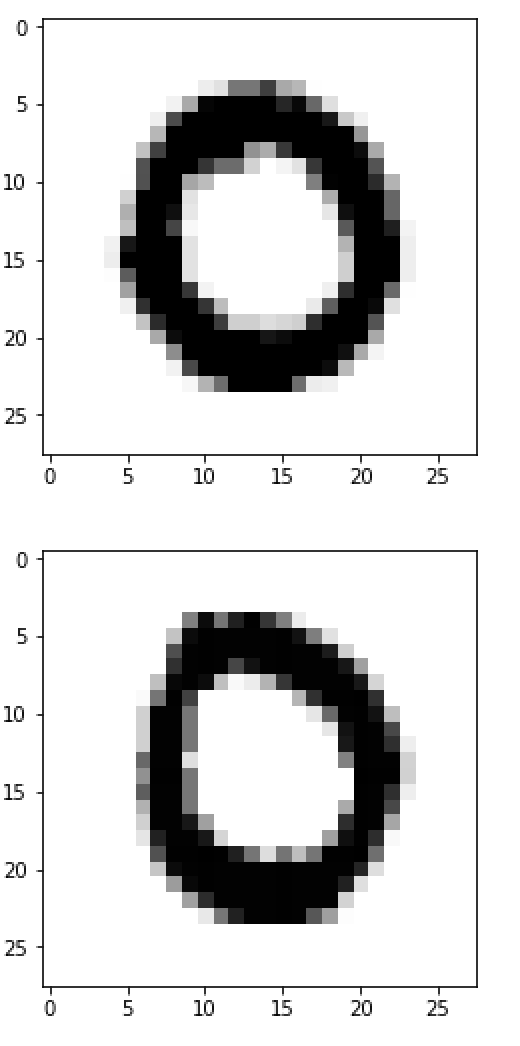
\includegraphics[width=30mm]{img/1-d/0.png}} &
      \addheight{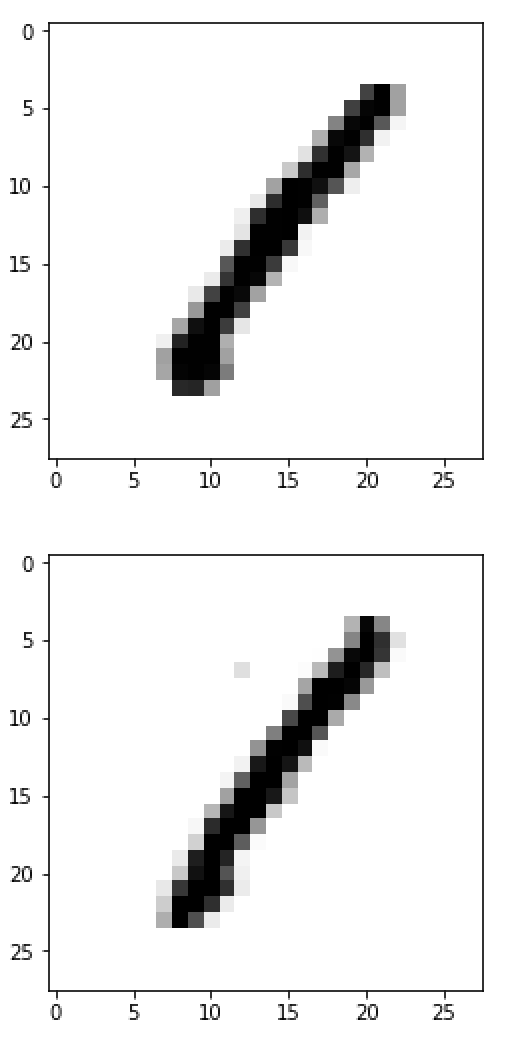
\includegraphics[width=30mm]{img/1-d/1.png}} &
      \addheight{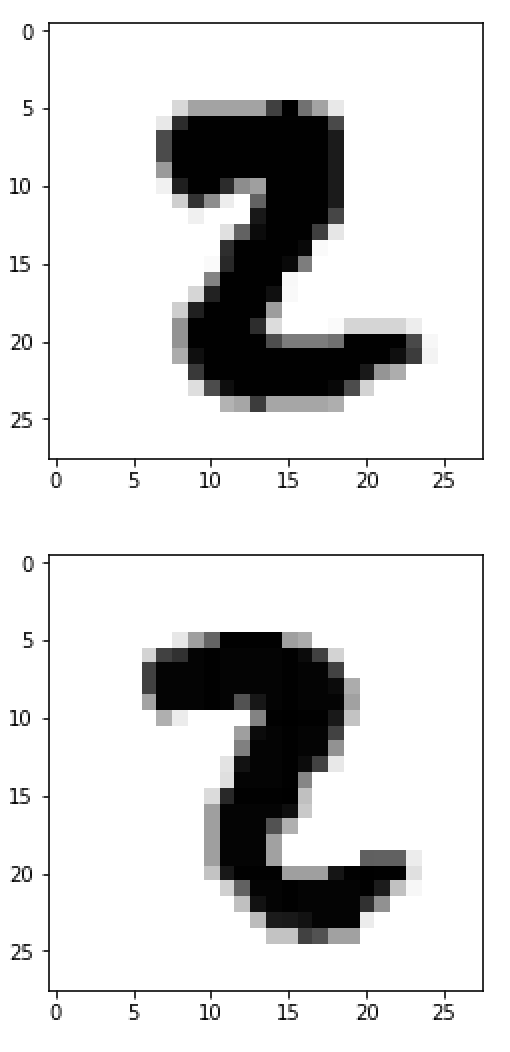
\includegraphics[width=30mm]{img/1-d/2.png}} &
      \addheight{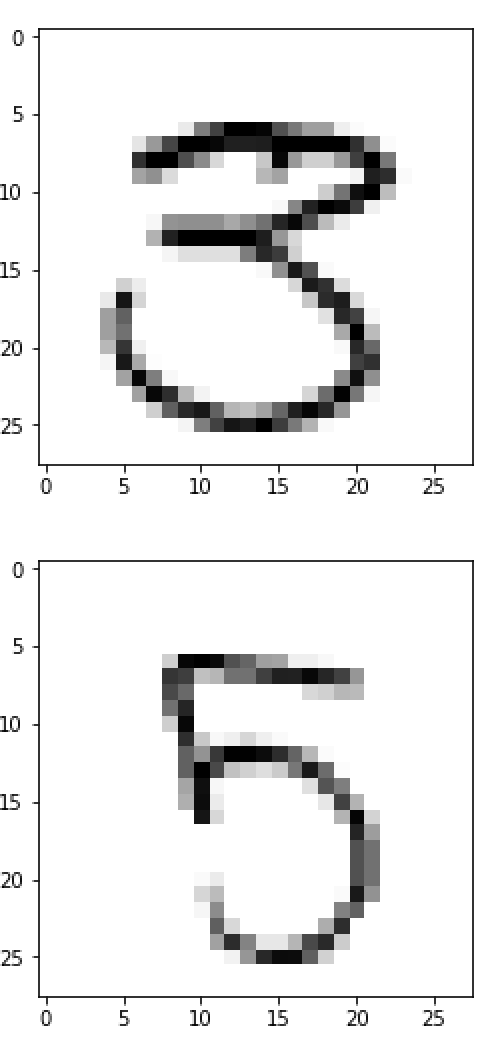
\includegraphics[width=30mm]{img/1-d/3.png}}* \\
      \addheight{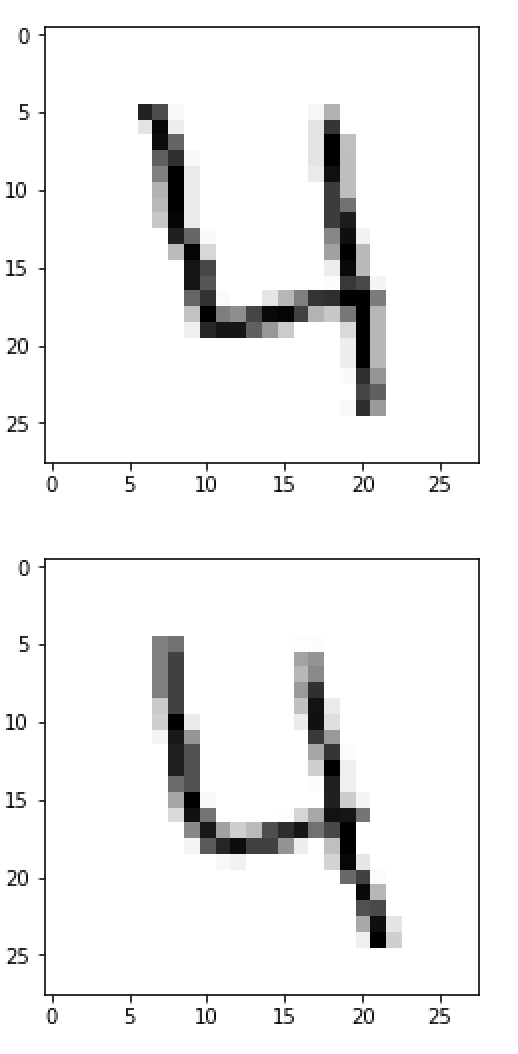
\includegraphics[width=30mm]{img/1-d/4.png}} &
      \addheight{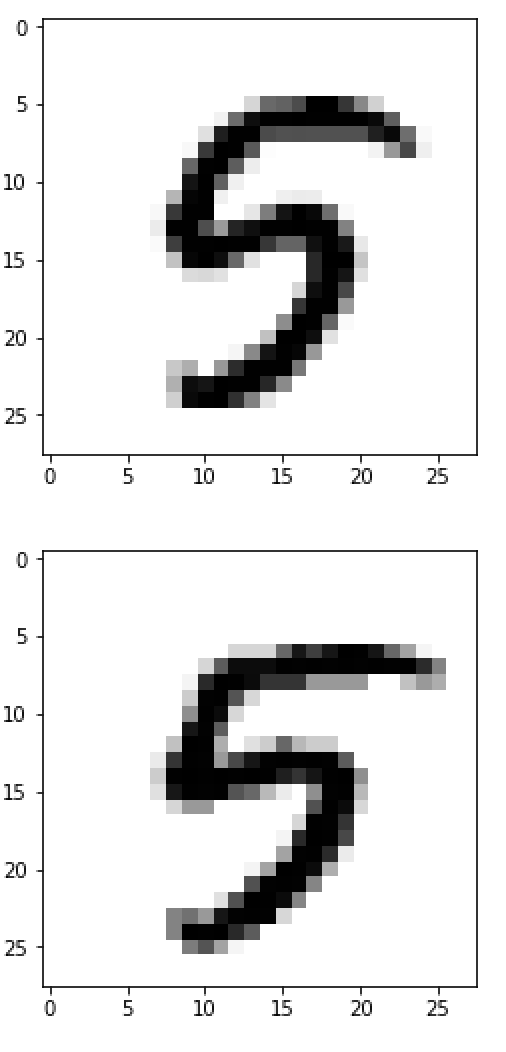
\includegraphics[width=30mm]{img/1-d/5.png}} &
      \addheight{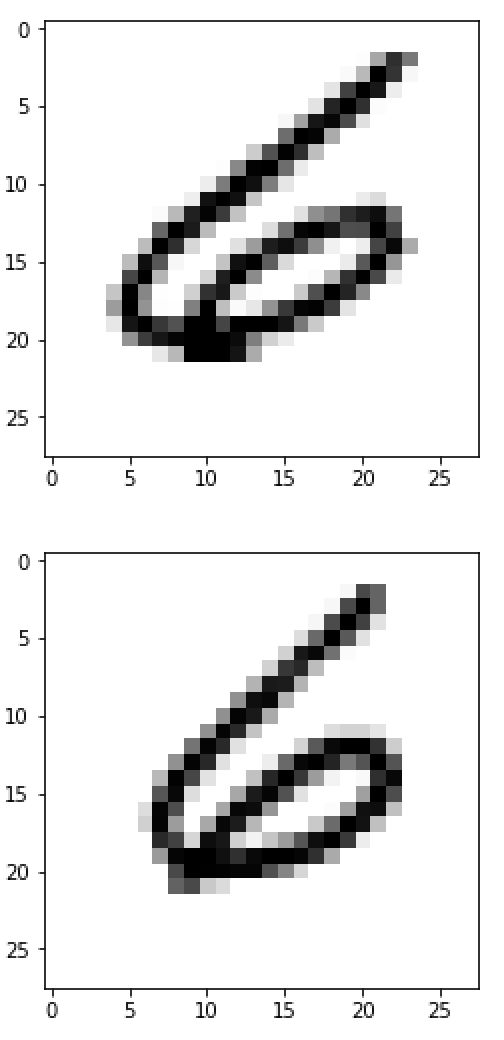
\includegraphics[width=30mm]{img/1-d/6.png}} &
      \addheight{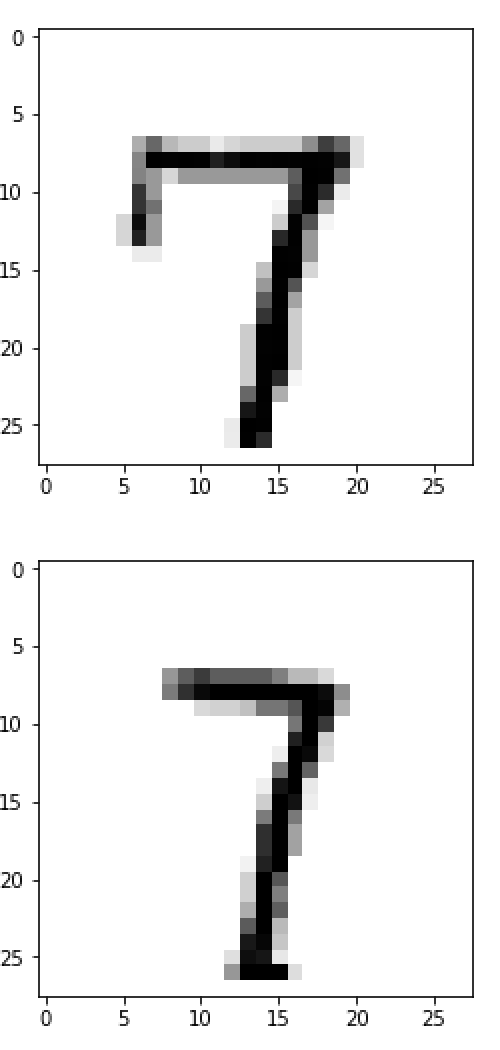
\includegraphics[width=30mm]{img/1-d/7.png}} \\
      \addheight{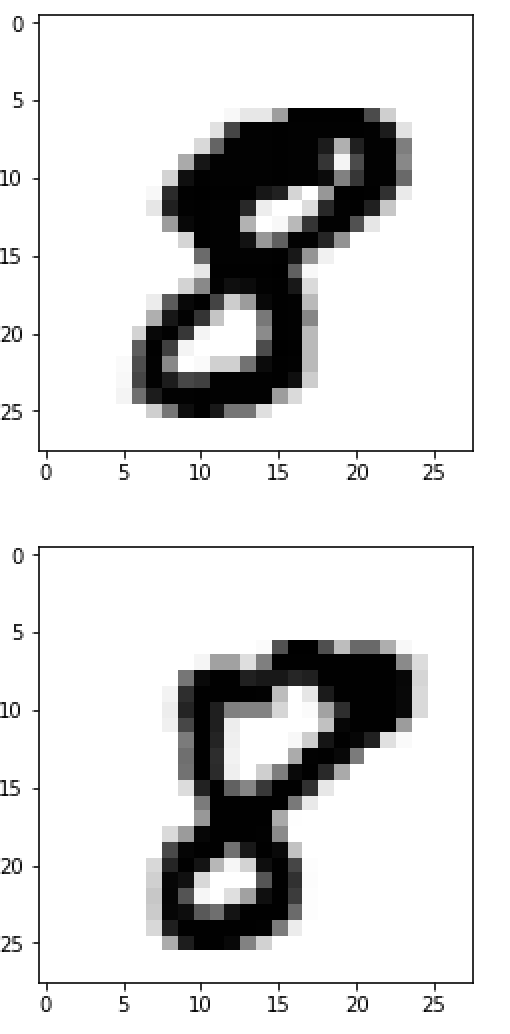
\includegraphics[width=30mm]{img/1-d/8.png}} &
      \addheight{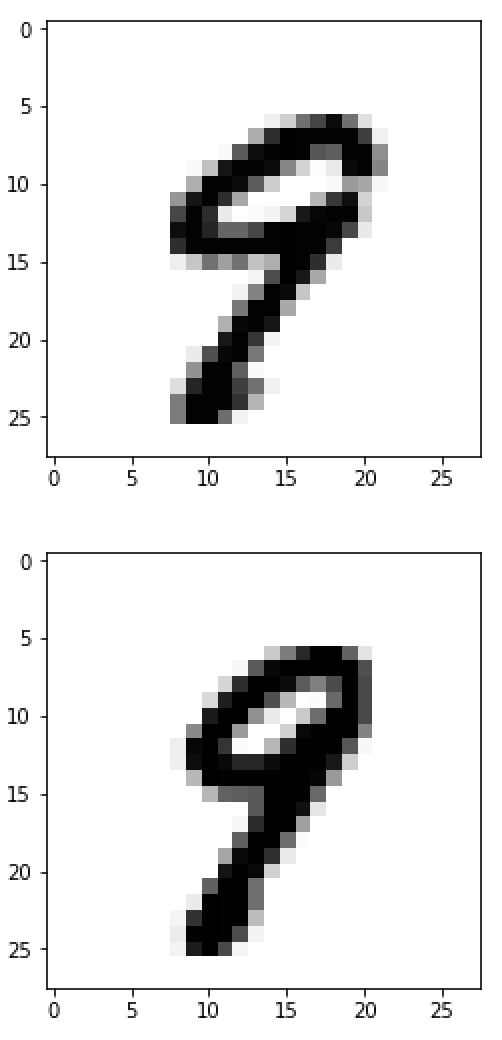
\includegraphics[width=30mm]{img/1-d/9.png}} \\
      \hline
\end{tabular}

\newpage
\subsection{e) Consider the case of binary comparison between the digits 0 and 1. Ignoring all the other digits, compute the pairwise distances for all genuine matches and all impostor matches, again using the L2 norm. Plot histograms of the genuine and impostor distances on the same set of axes.}
To get the genuine matches distances array, it necessary to call the function named \textbf{getGenuineMatches(digit1, digit2, labels, data)}, this function calculate the $L_2$ distance between all of the genuine matches in the data. The first 2 attributes in this exercise should be 0, and 1 because those are the 2 digits that we are using now but this function is able to do the same with different pairs of values. For the impostors matches distances, there is a function called \textbf{getImpostorMatches(digit1, digit2, labels, data)}, which is the same as the other but only for the impostors. Then to plot the data there is a function called \textbf{displayDoubleHistogram(array1, array2, label1, label2)} this will generate the graph showed below.

\begin{figure}[ht!]
\centering
\fbox{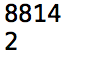
\includegraphics[scale=0.8]{img/1-e.png}}
\caption{Genuine Matches vs Impostor Matches}\label{Genuine vs Impostor}
\end{figure}

\newpage
\subsection{f) Generate an ROC curve from the above sets of distances. What is the equal error rate? What is the error rate of a classifier that simply guesses randomly?}
To generate the ROC curve, there is a function called \textbf{getAndDisplayROCCurve(genuine, impostors)}, this method calculate the probabilities of false positive, the probability of true positives and plot the ROC curve with the curve between 1.0 - 1.0. Then the equal error rate is the intersection between the 2 curves, its posible to see it in the figure below.
$$EER \approx 0.793$$
If simply guesses randomly, that means that the algorithm is not even look at the training data, but will just choose 0 or 1. So the error rate will be $50\%$. Below there is the ROC curve graph.

\begin{figure}[ht!]
\centering
\fbox{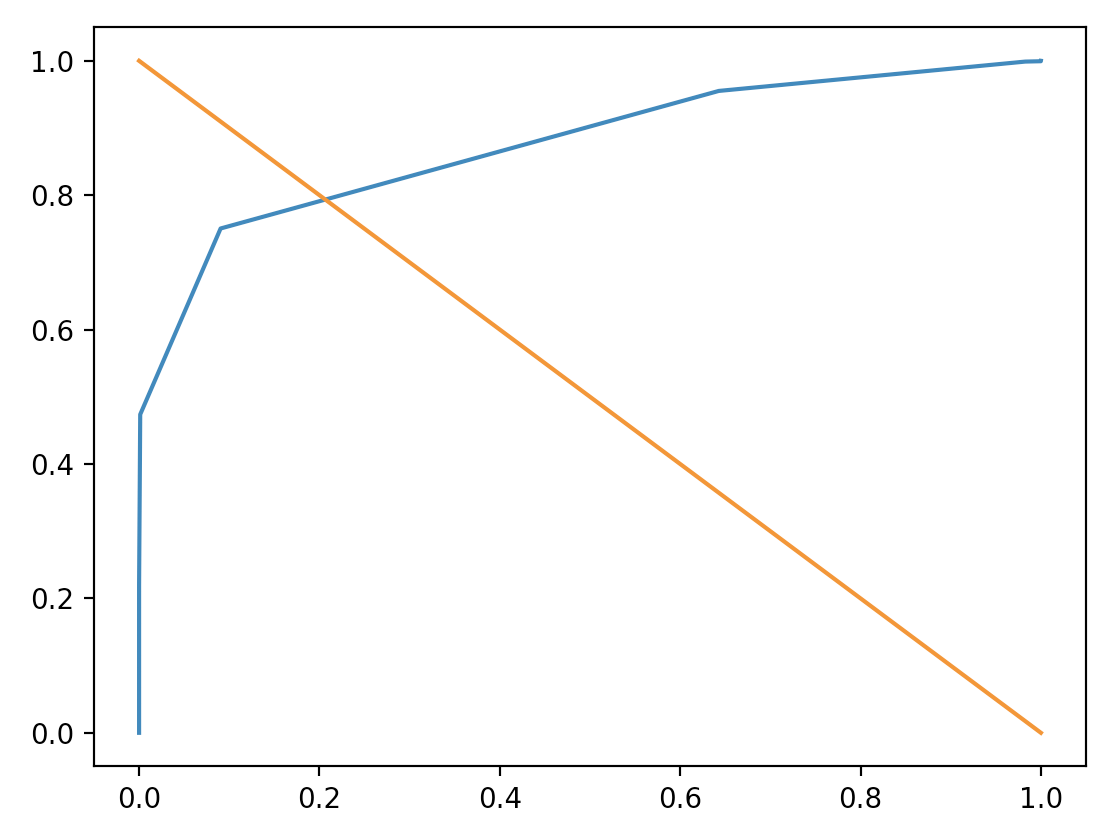
\includegraphics[scale=0.6]{img/1-f.png}}
\caption{ROC Curve for the sets of 0 and 1}\label{ROC Curve}
\end{figure}

\subsection{g) Implement a K-NN classifier. (You cannot use external libraries for this question; it should be your own implementation.)}
Implement the k-nearest neighbor at this point is easy. We already have the function that get the nearest neighbor. This means just a little adjustment to that one. This new one is called \textbf{getKNearestNeighbours(k, digit, train\_data)}. It creates an array of results, then each time that a new distance is lower that the lowest at that moment. This new item will replace the oldest item added to the array. At the beginning the array will start full of zeros. Then the function that implements the classifier is one called \textbf{kNearestNeighboursClassifier(k, train\_data, train\_labels, test\_data)}, this function  evaluates get the k nearest neighbor for each element of the test data. Then it calculate the votes and add the results to an array of labels. Then returns the array of labels of the test data.

\subsection{h) Using the training data for all digits, perform 3 fold cross-validation on your K-NN classifier and report your average accuracy.}
There is a function called \textbf{threeFoldCrossValidationKNN(k, data, labels)}, this function does all the work. Basically it divided the data into 3 arrays each of the same size. Then  runs the function \textbf{accuracyPercentage(testLabels, realLabels)}, for each sub array as the test and the other two as the train data. At the end it returns the average accuracy percentage of the three sub arrays. The function \textbf{accuracyPercentage(testLabels, realLabels)} receive the original labels of each sub array and also the labels returned by the classifier and evaluates the percentage of accuracy between them. In the end the result was:
$$\approx 95.1667\%$$

\subsection{i) Generate a confusion matrix (ofsize 10 x 10) from your results. Which digits are particularly tricky to classify?}
To generate the confusion matrix, first is needed to run the KNN classifier. After that there is a function called \textbf{generateConfusionMatrix(real\_labels, predicted\_labels)}. Is just necessary to call this function with the results of the KNN and the real labels. This method create the matrix evaluating both arrays and adding one to that item in the matrix. After this method there is a method called \textbf{printMatrix(matrix)}, this method show the matrix in an easy understandable way. By looking at the results that are showed below we can recognize that number 8 and 3 are the most tricky to get. They can be confused with any other number. Also we can review that the number 4 is easy to be confused with the number 9 because the biggest wrong amount of mistakes is 130 and is between 4 and 9. Below there are the results.

\begin{figure}[ht!]
\centering
\fbox{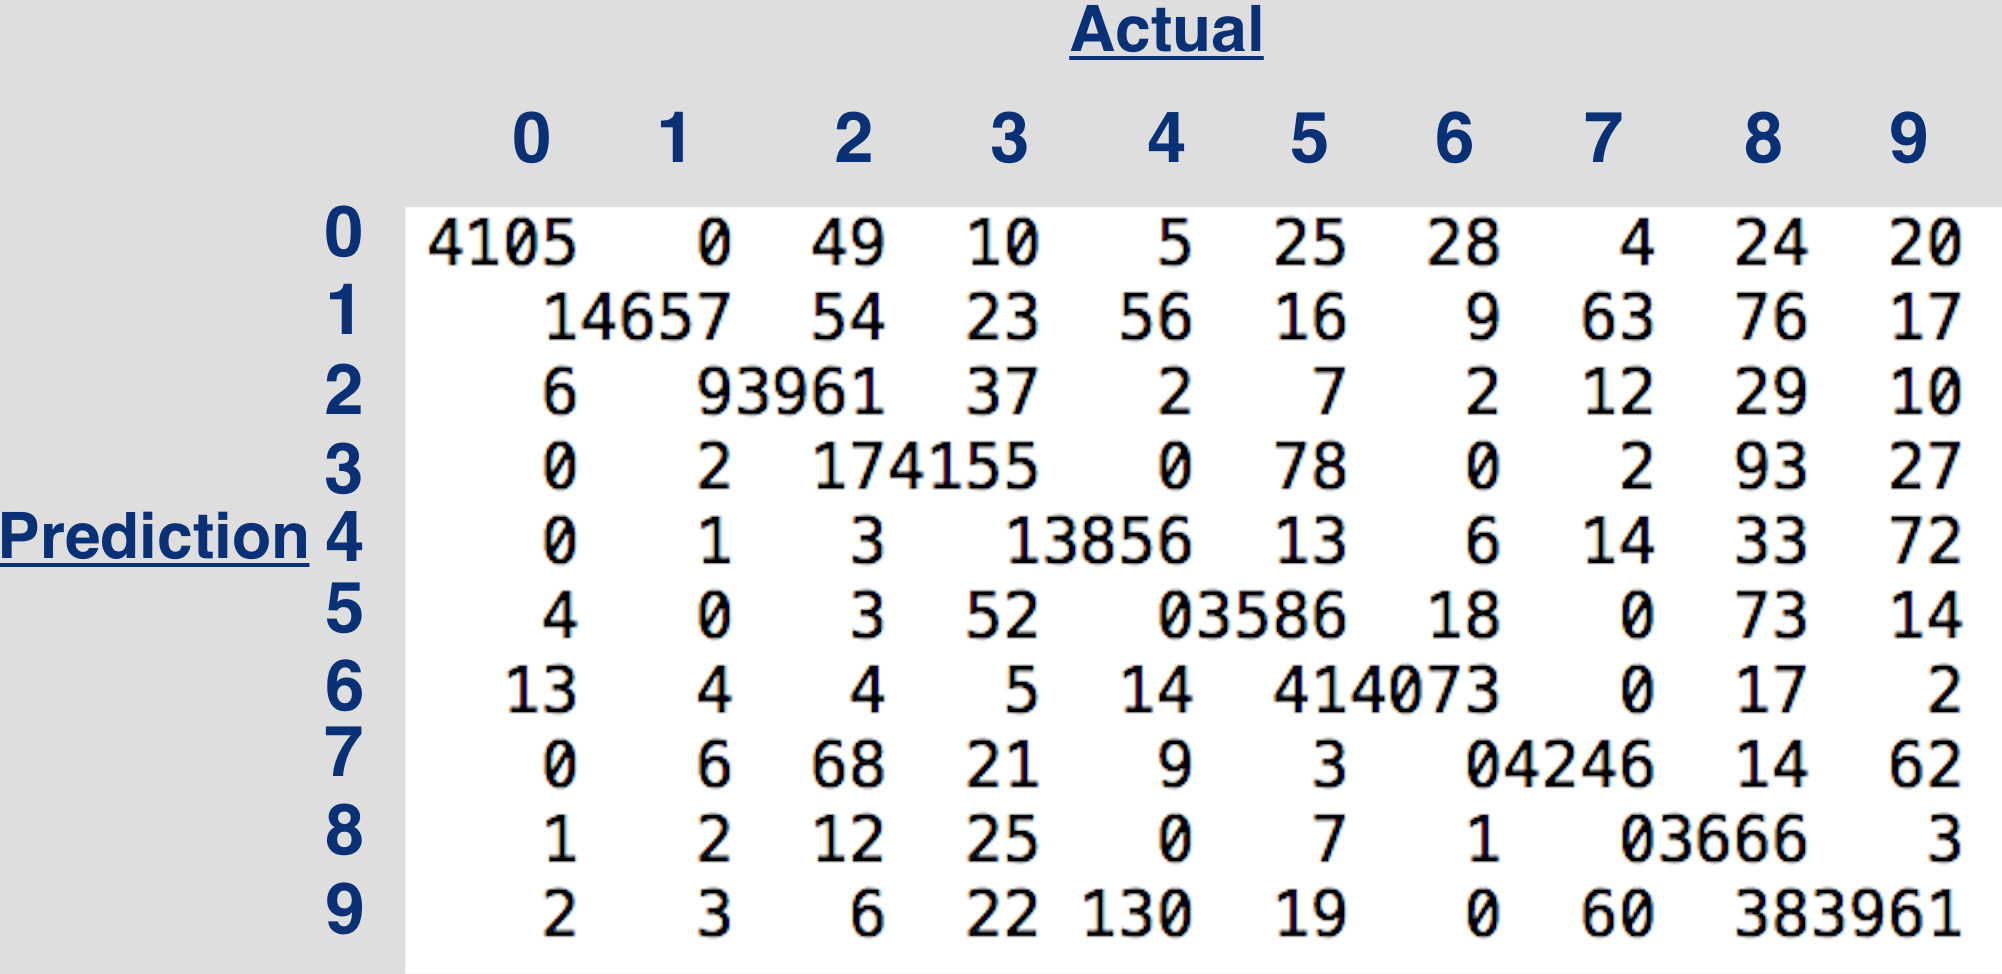
\includegraphics[scale=0.4]{img/1-i.png}}
\caption{Confusion Matrix}\label{Confusion Matrix}
\end{figure}

\section{The Titanic Disaster}
For the Titanic classification problem, we used inbuilt logistic regression classifier from scikit learn library. The first step was to prepare the data so that we can use it to train our classifier. In order to prepare the data, we have to convert few of the variables of the feature vector (gender, embark) to an integer type categorical variable and use average values for some variables for which data was absent.  We eventually used P-class, Sex, Age, SibSp, Parch, Fare and Embarked variables to train the data. We also used cross-validation to iterate over the various combinations of the variables to find the set of variables that has the maximum accuracy over the training data set. Once, we find the combination of the variable, we used that to generate the result file for the test dataset. We eventually submitted our results on the Kaggle and got 6900 rank and 75\% accuracy rate.

\section{Written Exercises}
\subsection{Variance of a sum. Show that the variance of a sum is $var[X-Y]=var[X] + var[Y] - 2*cov[X,Y]$, where $cov[X,Y]$ is the covariance between random variables $X$ and $Y$.}
$$ Var(X-Y) = E[(X-Y)^2] - E[X-Y]^2$$
$$ = E[X^2+Y^2 - 2XY] - [E(X)-E(Y)]^2$$
$$ = E[X^2]+E[Y^2]-2E[XY] - ([E(X)^2+E(Y)^2-2E[X]E[Y])$$
$$ = E[X^2] - E[X]^2 +E[Y^2]- E[Y]^2- 2(E[XY] - 2E[X]E[Y])$$
$$ = Var(X) + Var(Y) - 2 COV(X,Y)$$

\subsection{Bayes rule for quality control. You’re the foreman at a factory making ten million widgets per year. As a quality control step before shipment, you create a detector that tests for defective widgets be- fore sending them to customers. The test is uniformly 95\% accurate, meaning that the probability of testing positive given that the widget is defective is 0.95, as is the probability of testing negative given that the widget is not defective. Further, only one in 100,000 widgets is actually defective.}
\textbf{a) Suppose the test shows that a widget is defective. What are the chances that it’s actually defective given the test result?} \\\\
Let D be the event that the widget is actually defective and 
$$ P(D) = 0.00001 $$
Let A be the event that the detector classifies the widget as defective
$$ P(A|D) = 0.95 $$
$$ P(\bar{A}|\bar{D}) = 0.95 $$
$$ P(A|\bar{D}) = 0.05 $$
$$ P(\bar{A}|{D}) = 0.05 $$
$ P(D|A) = $ it is the probability that the widget is actually defective when it is classified as  'defective' by the detector
$$ P(D|A) = \frac{P(D\cap A)}{P(A)} = \frac{P(D)P(A|D)}{P(A)} $$
$$ = \frac{(0.00001) * (0.95)}{P(A|D)P(D) + P(A|\bar{D}) P(\bar{D})} $$
$$ = \frac{(0.00001) * (0.95)}{0.95*0.00001 + 0.05*0.99999} $$
$$ = 0.01\% $$

\textbf{b) If we throw out all widgets that are defective, how many good widgets are thrown away per year? How many bad widgets are still shipped to customers each year?} \\\\
Number of good widgets thrown per year = total number of widgets *$ P(\bar{D})* P(A|\bar{D})$\\
$$ P(\bar{D})*P(A|\bar{D}) = 0.99999 * 0.05 $$\\
Number of widgets = 10,000,0000 \\
Number of good widgets thrown per year $= 0.99999 * 0.05 * 10,000,0000$\\
$$= 499,995$$\\
Number of bad widgets given to customer per year = total number of widgets *$ P(D)* P(\bar{A}|D)$\\
$$ P(D)* P(\bar{A}|D) = 0.00001 * 0.05 $$\\
Number of widgets = 10,000,0000 \\
Number of bad widgets given to customer per year $= 0.00001 * 0.05 * 10,000,0000$\\
$$= 5$$

\subsection{In k-nearest neighbors, the classification is achieved by majority vote in the vicinity of data. Sup- pose our training data comprises n data points with two classes, each comprising exactly half of the training data, with some overlap between the two classes.}

\textbf{a) Describe what happens to the average 0-1 prediction error on the training data when the neighbor count k varies from n to 1. (In this case, the prediction for training data point $x_i$ includes $(x_i , y_i)$ as part of the example training data used by kNN.)}\\\\
When the neighbour count k is n, the algorithm effectively predicts both the classes/labels (0,1) for the test cases with the probability of 0.5. Hence, the prediction error is 0.5.
When the neighbour count k is 1, the algorithm effectively predicts the label for the test case based on only one neighbour - the one that is nearest to the test case. The prediction error in that case will depend on the overlap between the two classes and the variable that is being predicted. The error will be high at the boundary between the two classes. In this case, there is ‘some’ overlap between the two classes -  assuming that ‘some’ refers to be less than $<20\%$, the error rate will be lower than the error rate that we encounter when the neighbor count is n. We feel the prediction error in that scenario will be smaller and should be closer to the overlap rate.\\\\

\textbf{b) We randomly choose half of the data to be removed from the training data, train on the remaining half, and test on the held-out half. Predict and explain with a sketch how the average 0-1 prediction error on the held-out validation set might change when k varies? Explain your reasoning.)}\\\\

Now the test set and training set are both taken from the ‘original’ training set. In that case, both the test set and training set have the same distribution.  
When the neighbour count k is $\frac{n}{2}$ (the maximum possible value), the algorithm effectively predicts both the classes/labels (0,1) for the test cases with the probability of 0.5. Hence, the prediction error is 0.5.
When the neighbour count k is 1, the algorithm effectively predicts the label for the test case based on only one neighbour - the one that is nearest to the test case. The prediction error in that case will depend on the overlap between the two classes and the variable that is being predicted. The error will be high at the boundary between the two classes. In this case, there is ‘some’ overlap between the two classes -  assuming that ‘some’ refers to be less than $<20\%$, the error rate will be lower than the error rate that we encounter when the neighbor count is $\frac{n}{2}$.
However, the error rate will be higher than any value of neighbor count that is less than $\frac{n}{4}$.\\\\

\textbf{c) We wish to choose k by cross-validation and are considering how many folds to use. Compare both the computational requirements and the validation accuracy of using different numbers of folds for kNN and recommend an appropriate number.)}\\\\
As we increase the number of folds, the size of our test data set decreases  and the maximum value of neighbor count  k you can choose decrease.  If the number of folds is f, the maximum value of neighbor count can be (n - $\frac{n}{f}$).

When the number of folds is f, the number of computations required to determine the optimum value of neighbor count c will be  $\frac{n}{f}*(n-\frac{n}{f})$ (which is proportional to $n^2$ and inversely proportional to f). The number of computations decreases as f increases.

When the number of folds is less, we overfit the curve. If we fit the model to the entire training set, the error will underestimate the true generalization error, which is the error one sees on new data drawn from the same distribution. 

If we increase the number of folds to too high a value, the model will underfit the curve. If the number of folds is equal to n, then there is only one data point and the model will only see one class in the training set. The validation accuracy will be the lowest.

So, the curve will be inverted “U” where validation error will be on Y-axis and number of folds on X-Axis.\\\\

\textbf{d) In kNN, once k is determined, all of the k-nearest neighbors are weighted equally in deciding the class label. This may be inappropriate when k is large. Suggest a modification to the algorithm that avoids this caveat.}\\\\
One appropriate modification will be to change the weights of each of the neighbouring points. We can choose to give the nearby points higher weights than the farther points. This will ensure that the nearby points have higher say in deciding the class of the point.\\\\

\textbf{e) Give two reasons why kNN may be undesirable when the input dimension is high.}
\begin{itemize}
	\item It becomes computationally very intensive. kNN is a lazy learning algorithm. It computes the distance between the point whose class has to be predicted and all the points to identify the point’s k nearest neighbour. This computation of distance will be very resource intensive if the dimensionality is very high and the computation of the distance is dependent on all the dimensions.
	\item kNN gives equal value to all the dimensions in the feature vector. Some dimensions may be more relevant than others. This is also a problem.

\end{itemize}


% ============= FIN DE DOCUMENTO ==============
\end{document}

% % ················ IMAGEN ·················
% \begin{figure}[ht!]
% \centering
% \fbox{\includegraphics[scale=0.6]{img/flujo.png}}
% \caption{Flujo de caja anual}\label{flujo}
% \end{figure}
% %··········································

% % ················ IMAGEN DOBLE ·················
% \begin{figure}[ht!] \centering
% \subfloat[Esquemático]{\includegraphics[scale=0.44]{img/seguidor.png}}
% \subfloat[Simulación]{\includegraphics[scale=0.45]{img/seguidor1.png}}
% \caption{Simulación como seguidor de voltaje}\label{seguidor}
% \end{figure}
% %··········································